\documentclass[]{aastex6}
\usepackage{amsmath}
%\graphicspath{ {images/} }

\newcommand{\MOSES}{\textit{MOSES}}

\begin{document}


	\title{Determining Spectral Content of MOSES Images}
	\author{Jake Parker}
	\affil{Montana State University}
	\email{jacobdparker@gmail.com}
	
\begin{abstract}
The \textit{MOSES} (\textit{Multi-Order Solar EUV Spectrograph})  sounding rocket was launched February 8th, 2006 to capture images of the sun at 304 \AA. The \textit{MOSES} concave grating forms solar images in multiple spectral orders, in an effort to measure line profiles from a single exposure over a wide field of view. We present a preliminary identification of spectral content in \textit{MOSES} images. The cross correlation of subtracted images provide evidence of spectral content besides the normal 304 \AA \ He II line. We place confidence on the peaks in correlation by cross correlating random data that is statistically representative of \textit{MOSES} data. These significant peaks indicate a contribution to intensity from several coronal lines.  These lines are individually weak, but if not taken into account, they would significantly increase the residuals when inverting \textit{MOSES} images to obtain spectra.

\end{abstract}
\keywords{MOSES, Slitless Spectrograph, Cross Correlation, EUV}

\section{Introduction}

\textit{MOSES} (Multi-Order Solar EUV Spectrograph) is a sounding rocket mission designed and built by Charles Kankelborg and students at Montana State University  \citep{Kan01}.  First launched in 2006, \textit{MOSES} gathered solar images using a slitless spectrograph with a passband centered around the He II 304 \AA \ spectral line.  Slitless spectrographs provide a unique view of the Sun by using a diffraction grating paired with detectors at both central and outboard orders. This paring allows \MOSES \ to capture spatial and spectral information simultaneously over a wide field of view.

\begin{figure*}[t]
\figurenum{1}
\centering
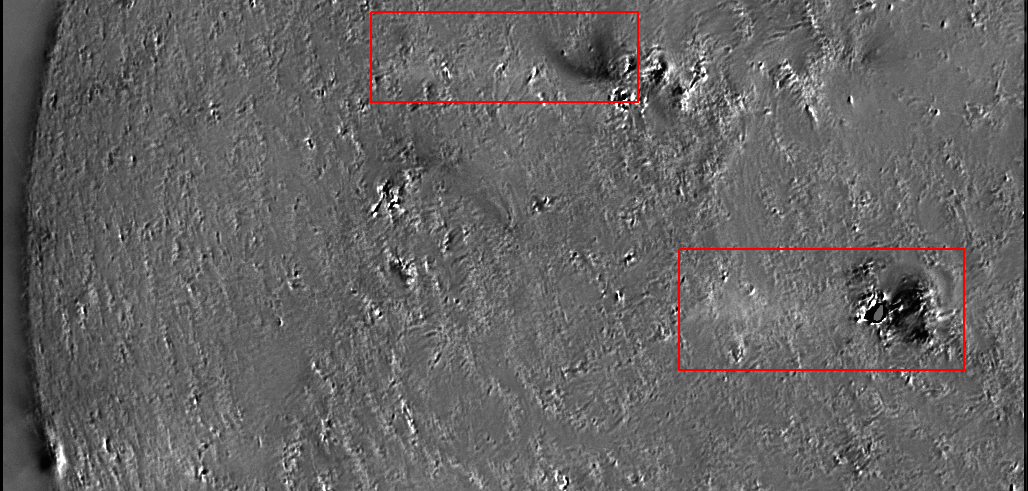
\includegraphics[scale=.4]{images/wishbone.png}
\caption{An image of MOSES zero order image subtracted from the plus one order image.  Dipolar structures give evidence of either Doppler shifted 304 objects or objects created by other spectral lines. Red boxes surround objects of questionable spectral content.  The upper box surrounds the ``wishbone''.}
\end{figure*}	

Subtracted a zero order images from an outboard order image provides evidence of extra spectral content in \MOSES \ images. Outboard order images from \textit{MOSES} were aligned to the central order by maximizing the cross correlation between each image. Subtracting one image from another removes most of the contributions from stationary objects in the dominate He II line. Remaining objects are cause by objects appearing in different locations in different orders.  This movement is caused by either by a Doppler shifted line or a different  than 304 \AA \ .  The the dispersion created by the diffraction grating is approximately 30 m\AA \ per pixel at the plus and minus order images.  At 304 \AA \ a one pixel shift corresponds to approximately 30 km/s Doppler shift.  Therefore any dipole separated by more than 10 pixels is most likely not He II. Figure 1 shows two red boxes surrounding dipolar objects with separation that is too great to be due to Doppler shifted He II objects.  We hope to identify the spectral lines contained in these objects by cross correlating subtracted \textit{MOSES} images and identifying peaks in correlation.

\begin{figure*}[t]
\figurenum{2}
\centering
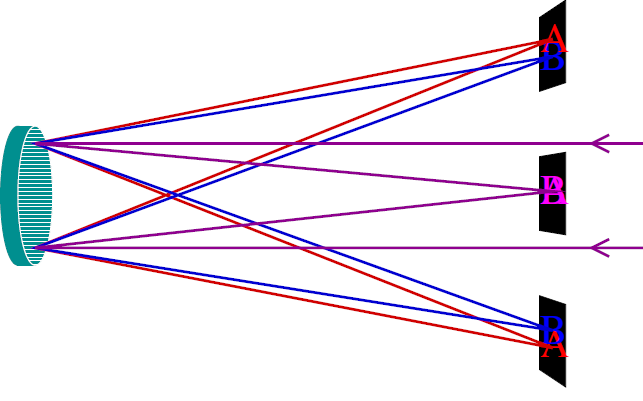
\includegraphics[scale=.5]{images/instrument.png}
\caption{This cartoon demonstrates how \textit{MOSES} separates incoming light into three separate images using a diffraction grating. Light incident on a concave primary mirror with grating (left) is then focused onto three different CCDs (right). This system also contains a secondary fold flat mirror not pictured.} 
\end{figure*}

Cross correlation functions of images are complex.  Peaks in correlation occur regularly and their significance is sometimes questionable.  We test the null hypothesis by correlating random data that is statically representative of \MOSES \ data.  This data was generated to resemble \textit{MOSES} images in power spectra and auto correlation.  We use image columns as the basis for random array generation because they contain information about the distribution of solar features and not wavelength dispersion. Unfortunately, a \MOSES column is not long enough to test the null hypothesis at large lag.  We solve this problem by increasing the resolution of our randomly generated columns in Fourier space.  Cross Correlating these randomly generated data places a confidence on whether or not a peak in correlation rejects the null hypothesis.   

Once we are able to reject the null hypothesis we need to identify what spectral information is contained in the cross correlation function.  An images cross correlation function in the dispersion direction depends on solar features and their wavelength, size, and intensity.  These solar features in He II images are a mixture of transition region features and coronal features. Coronal and transition images were captured \textit{EIT} (Extreme-ultraviolet Imaging Telescope) on the \textit{MOSES} launch day.  By taking the four EUV band images from EIT (171 \AA , 195 \AA , 284 \AA , and 304 \AA ) we create a forward model for \textit{MOSES}.  The forward model takes the input of line intensity.  Line intensity can then be tweaked until best fit with the \textit{MOSES} correlation function is achieved. These best fit intensities should be representative of the \textit{MOSES} image spectral content.  

\section{Methods and Results}

\subsection{MOSES Bandpass and EUV Spectra}   
	The \textit{MOSES} instrument has a pass band centered around 304 \AA \. The passband is defined by a narrow-band multilayer coating all mirrors \citep{Owens2005} as seen in Figure 3, and aluminum filters placed in front of the CCDs. Table 1 shows EUV spectral lines within the \MOSES \ passband \citep{Spec98} from a solar active region. Combining EUV line intensity with the throughput curve from Figure 3 and our aluminum filters we get a relative intensity of each line to 304 \AA \ He II.  Using line center for each EUV line we calculate the wavelength dispersion in pixels.  The dispersion is measured from and objects position in the central order.  The Fe XV and Fe XVII lines are on the far sides of our pass band but their relative intensity to 304 \AA \ is only half that of Si XI, an element we strongly suspected to see \MOSES \ images.  The two iron lines do have a large pixel dispersion but can still fall within a \MOSES \ image.  These bright EUV lines within \MOSES \ passband appear as features in the subtracted images and will negatively affect inversion.


\begin{figure*}[t]
\figurenum{3}
\centering
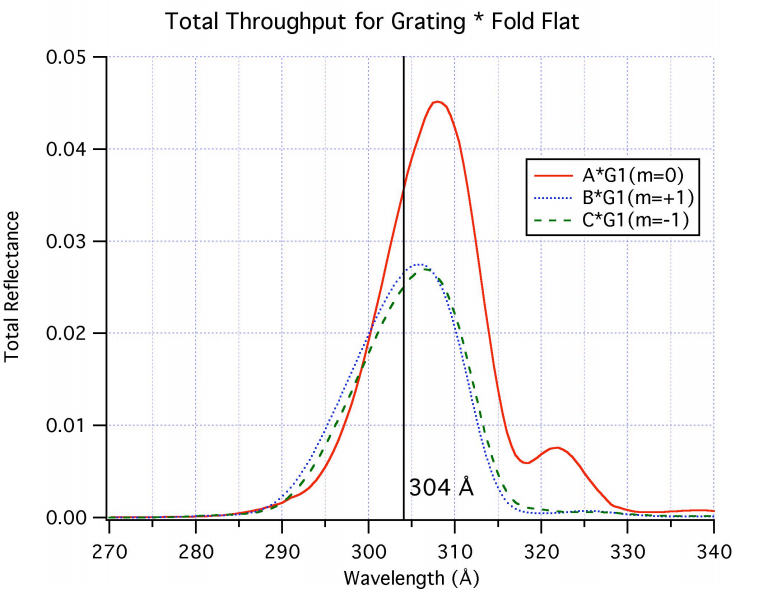
\includegraphics[scale=.5]{images/MOSES_throughput.png}
\caption{This figure from \citep{Owens2005} shows the optical throughput of the \textit{MOSES} instrument.}
\end{figure*}	



\begin{table}[htbp]
\caption{EUV Spectrum for active region sun  \citep{Spec98} combined with throughput \citep{Owens2005} to show relative intensities of spectral lines present in \textit{MOSES} images }
\resizebox{\columnwidth}{!}{%
\begin{tabular}{|l|r|r|r|r|r|}
\hline
Element & \multicolumn{1}{l|}{Wavelenth} & \multicolumn{1}{l|}{Intensitiy} & \multicolumn{1}{l|}{Intensity times} & \multicolumn{1}{l|}{Percent  HeII } & \multicolumn{1}{l|}{Pixel Shift} \\ \hline
 & \multicolumn{1}{l|}{(\AA)} & \multicolumn{1}{l|}{($ergs$\ $cm^{-2} s^{-1} sr^{-1}$)} & \multicolumn{1}{l|}{Throughput} & \multicolumn{1}{l|}{Intensity} & \multicolumn{1}{l|}{(from 304)} \\ \hline
Fe XV & 284.151 & 13900 & 55.71 & 4.58 & -650.0 \\ \hline
S XI & 285.82 & 132 & 0.59 & 0.05 & -594.8 \\ \hline
S XII & 288.415 & 203 & 1.56 & 0.13 & -508.8 \\ \hline
 & 288.588 & 102 & 0.78 & 0.06 & -503.1 \\ \hline
Fe XIV & 289.14 & 213 & 1.63 & 0.13 & -484.8 \\ \hline
Ni XVIII & 291.983 & 481 & 6.36 & 0.52 & -390.7 \\ \hline
Si IX & 292.756 & 126 & 1.95 & 0.16 & -365.1 \\ \hline
Si IX & 292.858 & 61.6 & 0.95 & 0.08 & -361.7 \\ \hline
Si IX + Fe VI & 296.102 & 179 & 3.93 & 0.32 & -254.3 \\ \hline
Si XI & 303.317 & 3360 & 113.46 & 9.33 & -15.4 \\ \hline
He II & 303.782 & 36000 & 1215.60 & 100.00 & 0.0 \\ \hline
Mn XIV (+Fe XV) & 304.868 & 216 & 7.50 & 0.62 & 36.0 \\ \hline
Fe XI + Fe VI & 308.545 & 120 & 4.38 & 0.36 & 157.7 \\ \hline
Fe XIII & 312.167 & 172 & 5.51 & 0.45 & 277.7 \\ \hline
Mg VIII & 315.029 & 144 & 3.78 & 0.31 & 372.4 \\ \hline
 & 317.023 & 62.1 & 1.18 & 0.10 & 438.5 \\ \hline
Fe XIII & 318.1 & 112 & 1.69 & 0.14 & 474.1 \\ \hline
Mg VII + Ni XV & 319.002 & 227 & 2.67 & 0.22 & 504.0 \\ \hline
Fe XIII & 320.796 & 195 & 1.15 & 0.09 & 563.4 \\ \hline
Al X  & 332.782 & 173 & 0.85 & 0.07 & 960.4 \\ \hline
Fe XIV & 334.167 & 923 & 3.43 & 0.28 & 1006.2 \\ \hline
Fe XVI & 335.401 & 12000 & 38.15 & 3.14 & 1047.1 \\ \hline
\end{tabular}}
\label{Label}
\end{table}




\subsection{Time Integration of MOSES Images}
	During it's flight in 2006 \textit{MOSES} took images with a variety of exposure lengths.  Longer exposures contain more information about dimmer features but are saturated in brighter active regions.  We are mostly concerned about bulk properties of the data set and not variations in features between exposures (which are minimal).  Therefore we have created a single image for all three orders that contain no saturated pixels by integrating through time.  We integrate exposures through time by computing an effective exposure length for each image based on the median intensity and averaging all non saturated pixels through time. This averaging gives a single, smooth, non saturated solar image for each order. Having three time integrated \MOSES \ images gives us only two subtracted images to cross correlate. 

\subsection{Cross Correlation}
The discrete cross correlation is defined in the following way:

\begin{equation}
(x \otimes y) (z) \equiv \dfrac{ \sum_{n=0}^{N-z-1} (x_n-\bar{x})(y_{n+z}-\bar{y})   }{\sqrt{[\sum_{n=0}^{N-1} (x_n-\bar{x})^2][\sum_{n=0}^{N-1} (y_{n}-\bar{y})^2 ]}}.
\end{equation}

The cross correlation function has maximum value when the overlapping parts (defined by lag z) of two functions have the same form and a minimum when two overlapping functions are orthogonal. Figure 4 shows an example of the signal we are looking for in a simple 1-D representation of a solar feature as viewed by \MOSES.  

\begin{figure*}[t]
\figurenum{4}
\centering
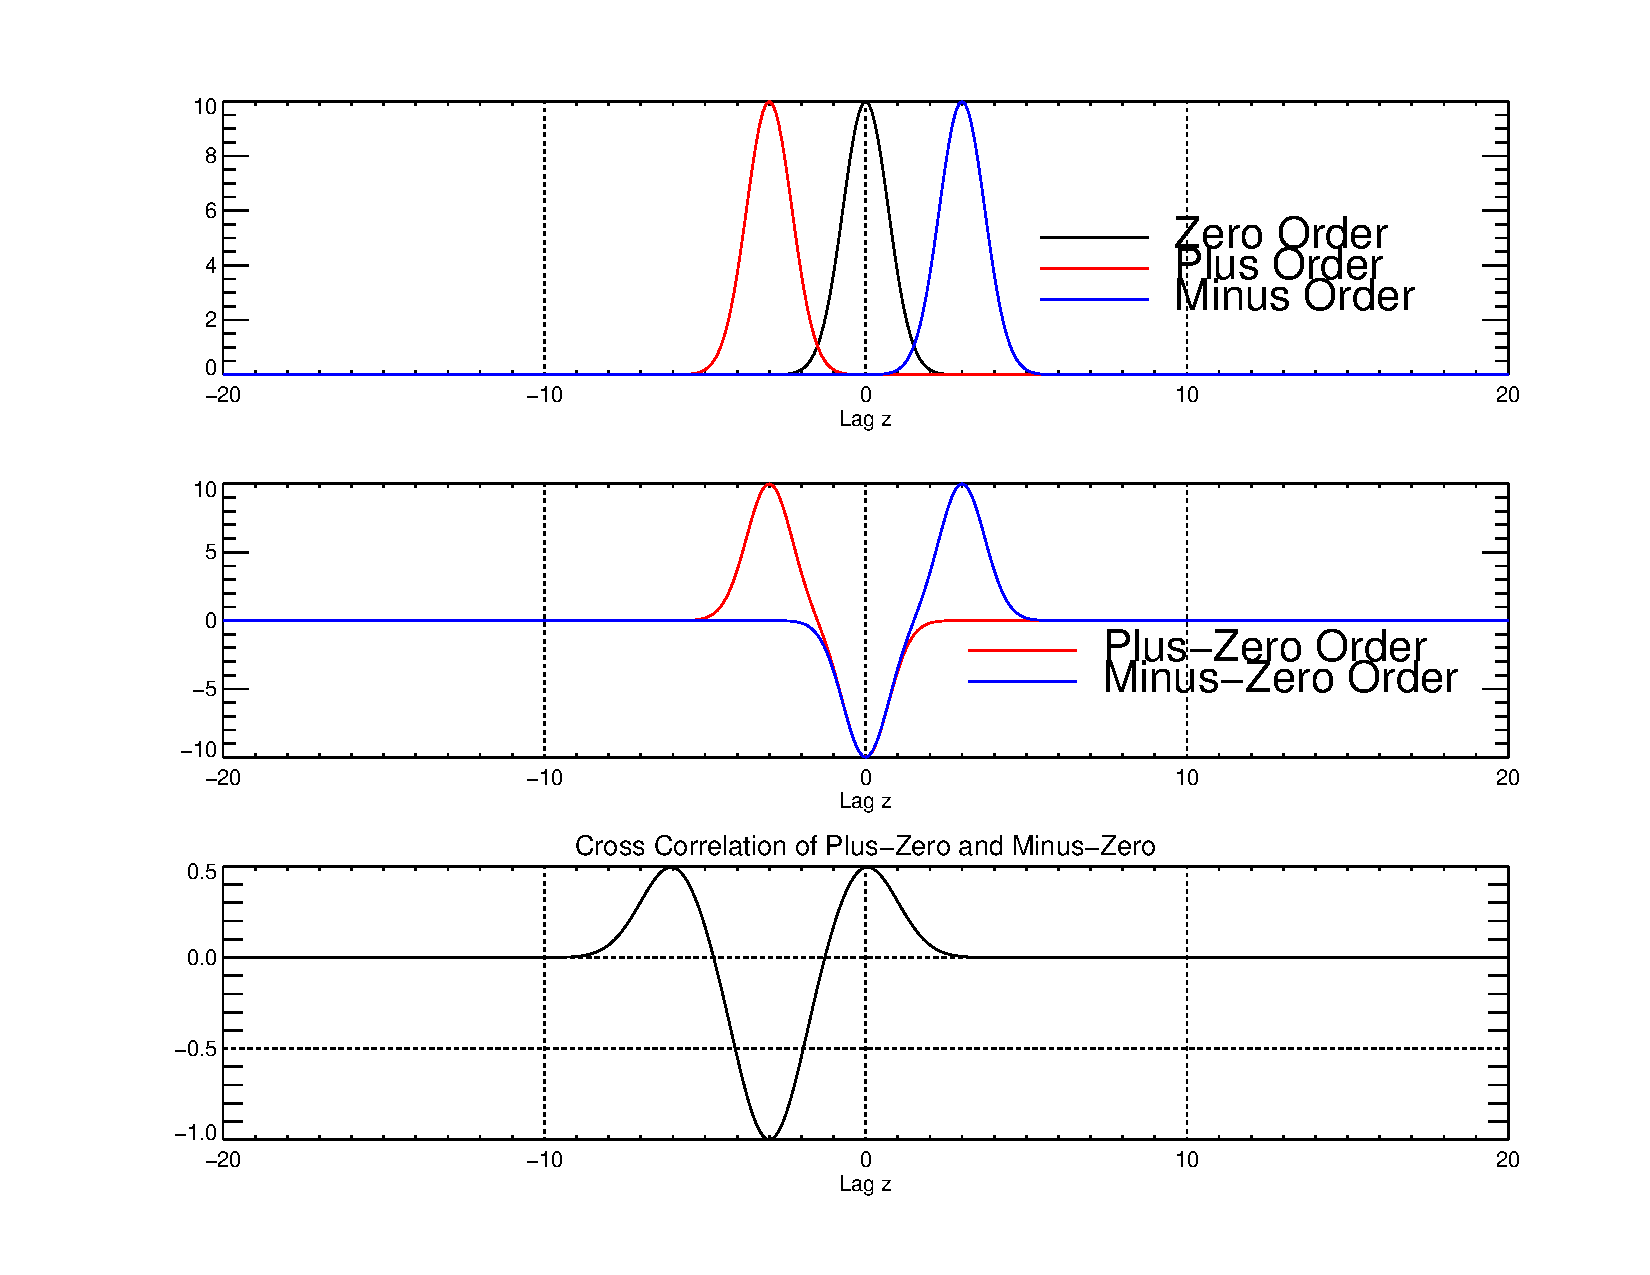
\includegraphics[scale=.5]{images/test1.pdf}
\caption{The top panel shows how an object not of He II would appear in a MOSES image. The object would appear in different locations in the Plus and Minus orders due to the diffraction grating.  The center panel shows subtracted images.  The Bottom panel shows the cross correlation of the subtracted image.}
\end{figure*}	

Unfortunately the Sun does not produce Gaussian objects of a single spectral line on a blank canvas. A \MOSES \ correlation function that contains more information and is therefore more cryptic. The blue curve in Figure 5 show correlation between the two subtracted \textit{MOSES} images. Significant features in the correlation function are key to identifying extra spectral content.

\begin{figure*}[t]
\figurenum{5}
\centering
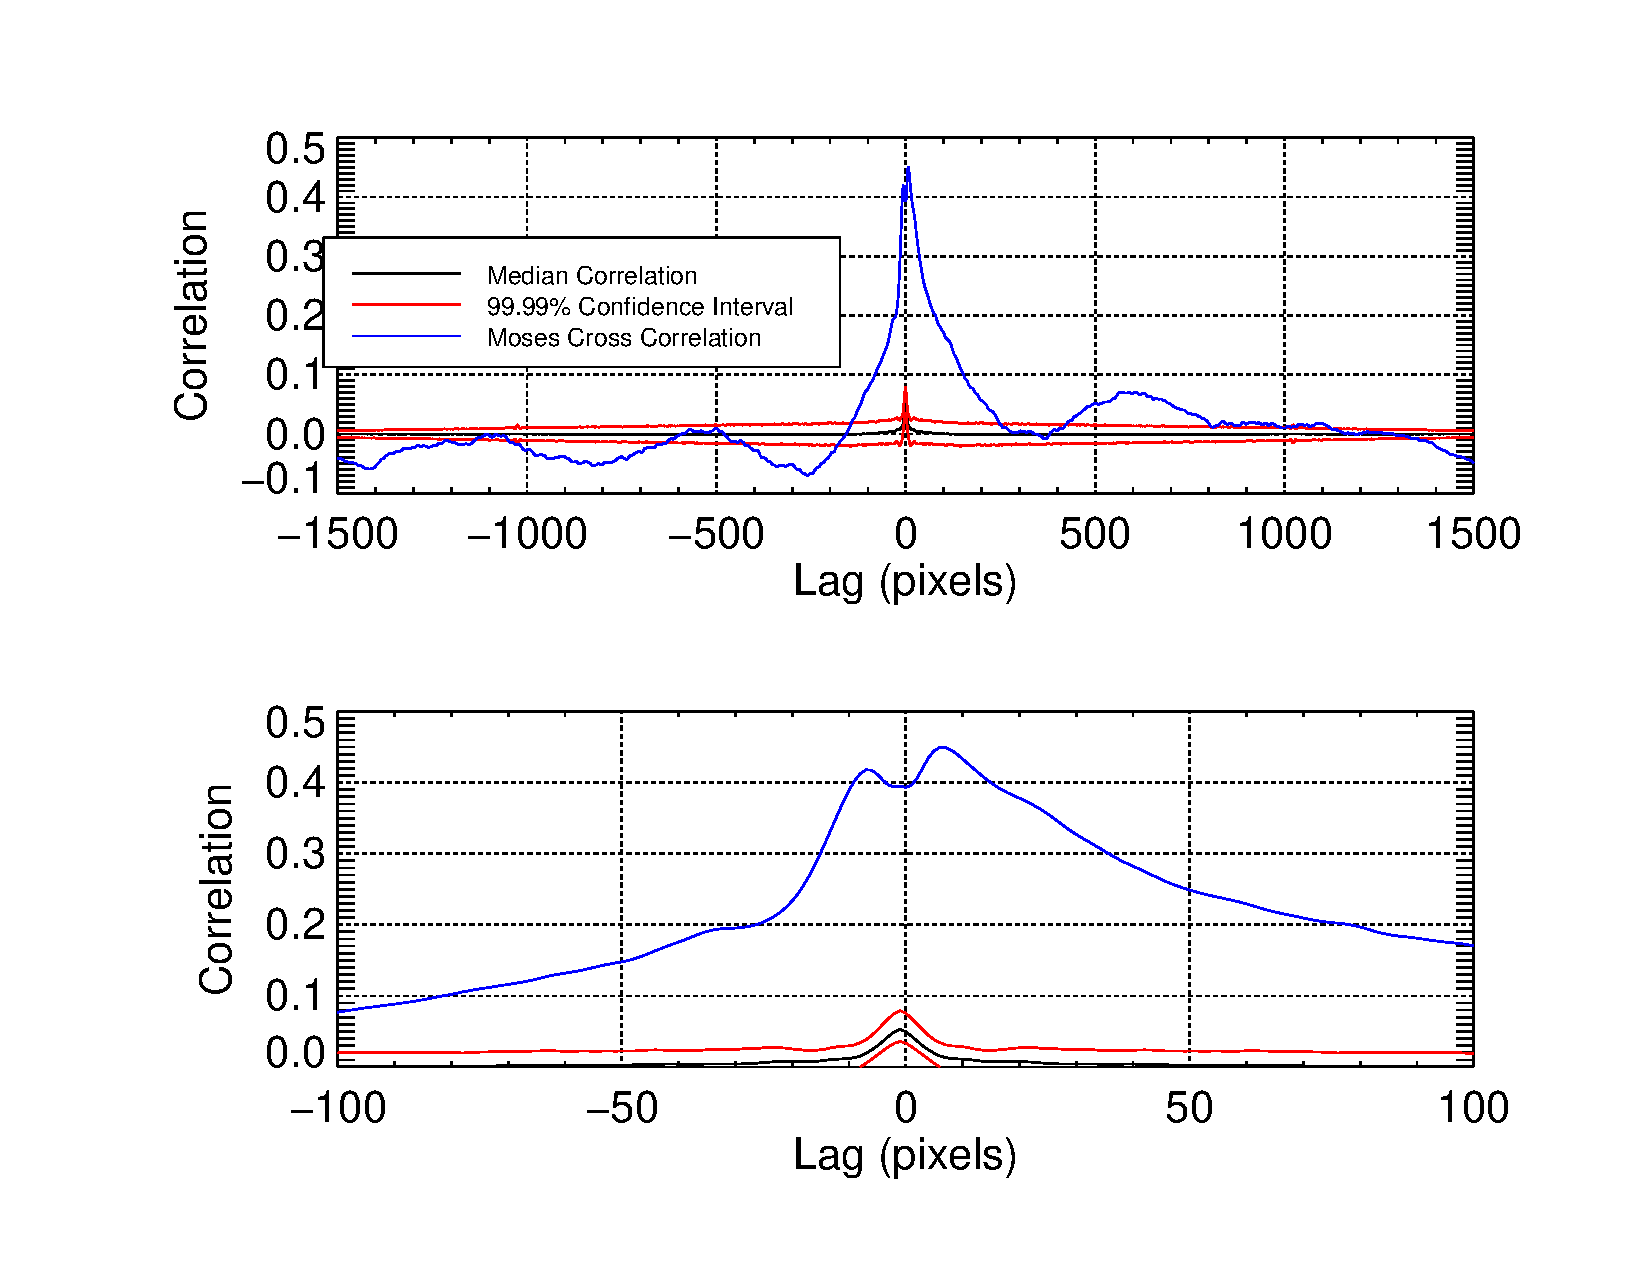
\includegraphics[scale=.5]{images/sigtest_5.pdf}
\caption{The blue curve is the actual cross correlation between the two time integrated \textit{MOSES} subtracted images.  The top red, middle black, and bottom red curves define the 99.995th , 50th , and .005th percentiles of the distribution of random correlations for a given lag with 5 degrees of freedom.}
\end{figure*}	


\subsection{Random Data Generation and Significance Testing}

\begin{figure*}[t]
\figurenum{6}
\centering
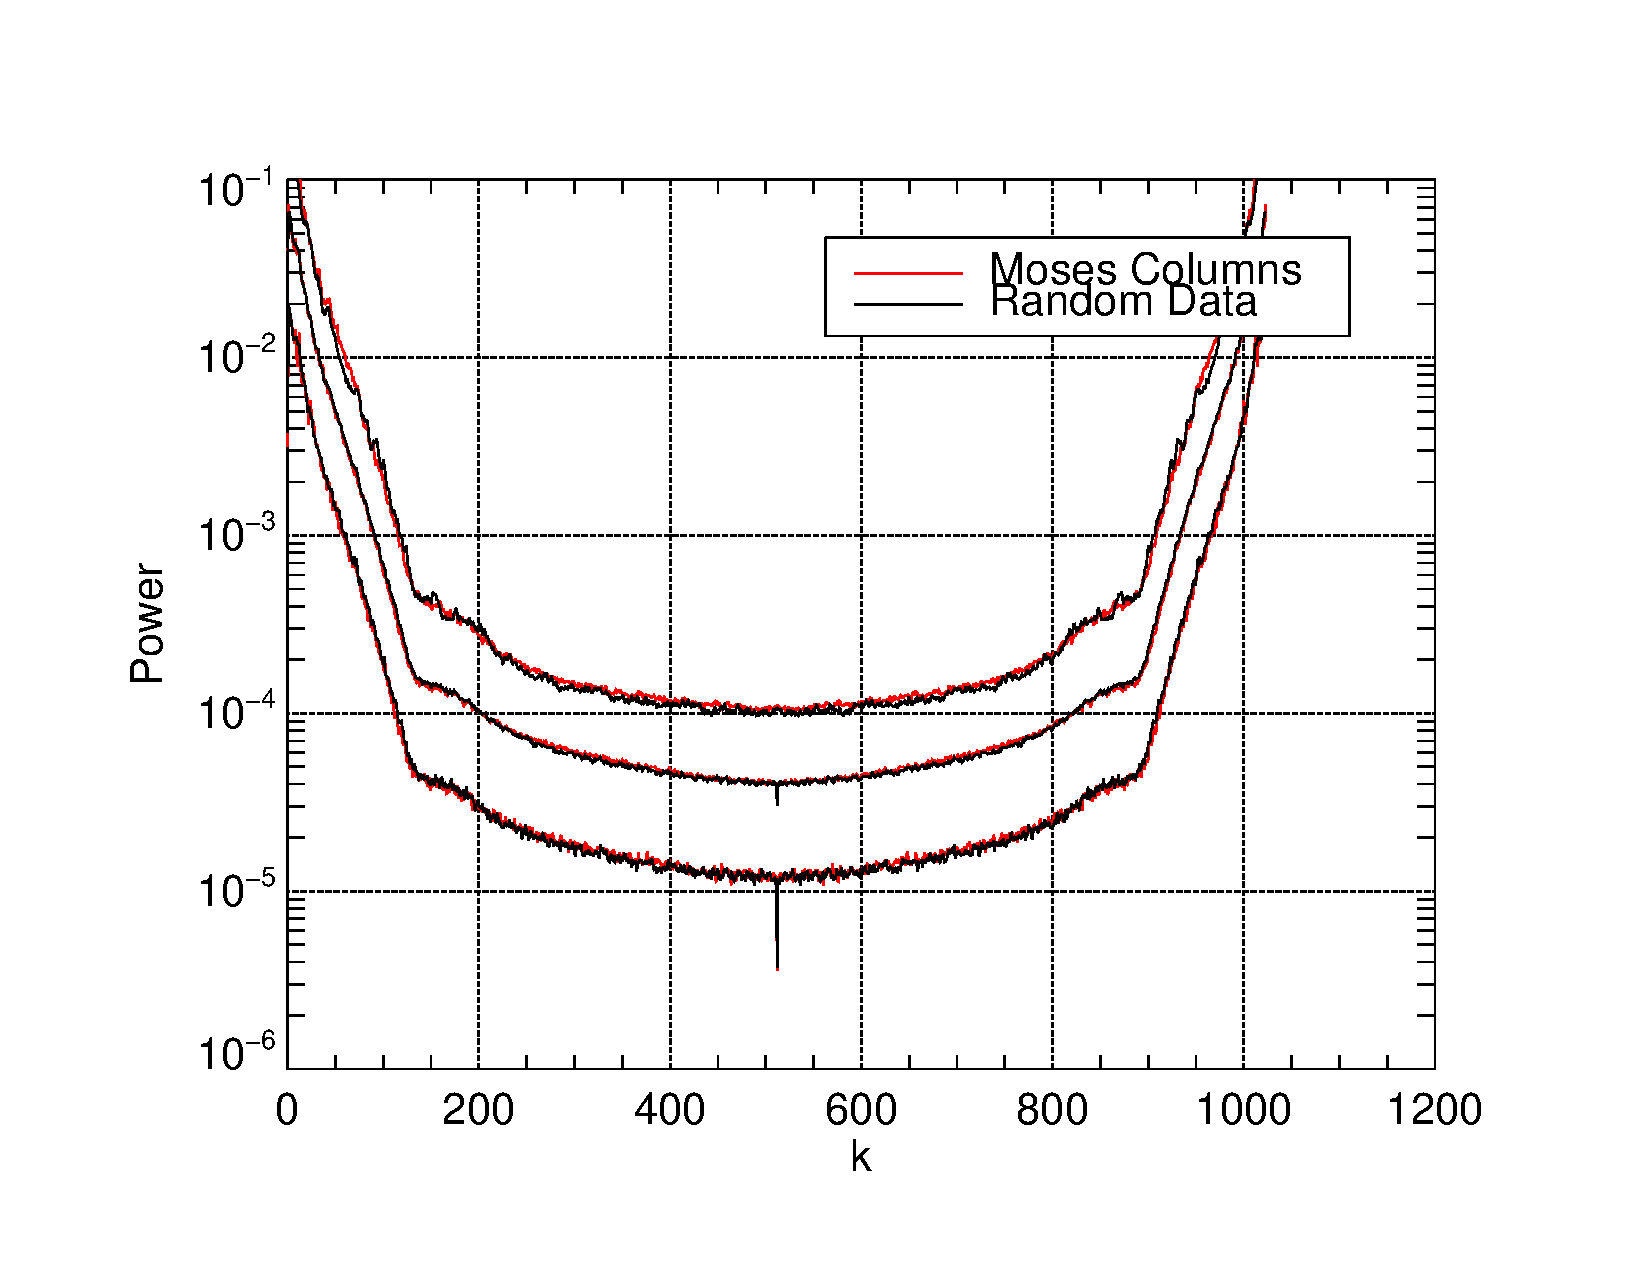
\includegraphics[scale=.5]{images/sigtestpower.pdf}
\caption{A comparison of the power spectra distribution for \textit{MOSES} columns and random 1024 long section of our random 2048 generated arrays.  The top, middle, and bottom curves define the 93.75th, 50th, and 6.25th percentiles of the distributions.  It has been verified that these curves align for other percentiles as well}
\end{figure*}	


\begin{figure*}[t]
\figurenum{7}
\centering
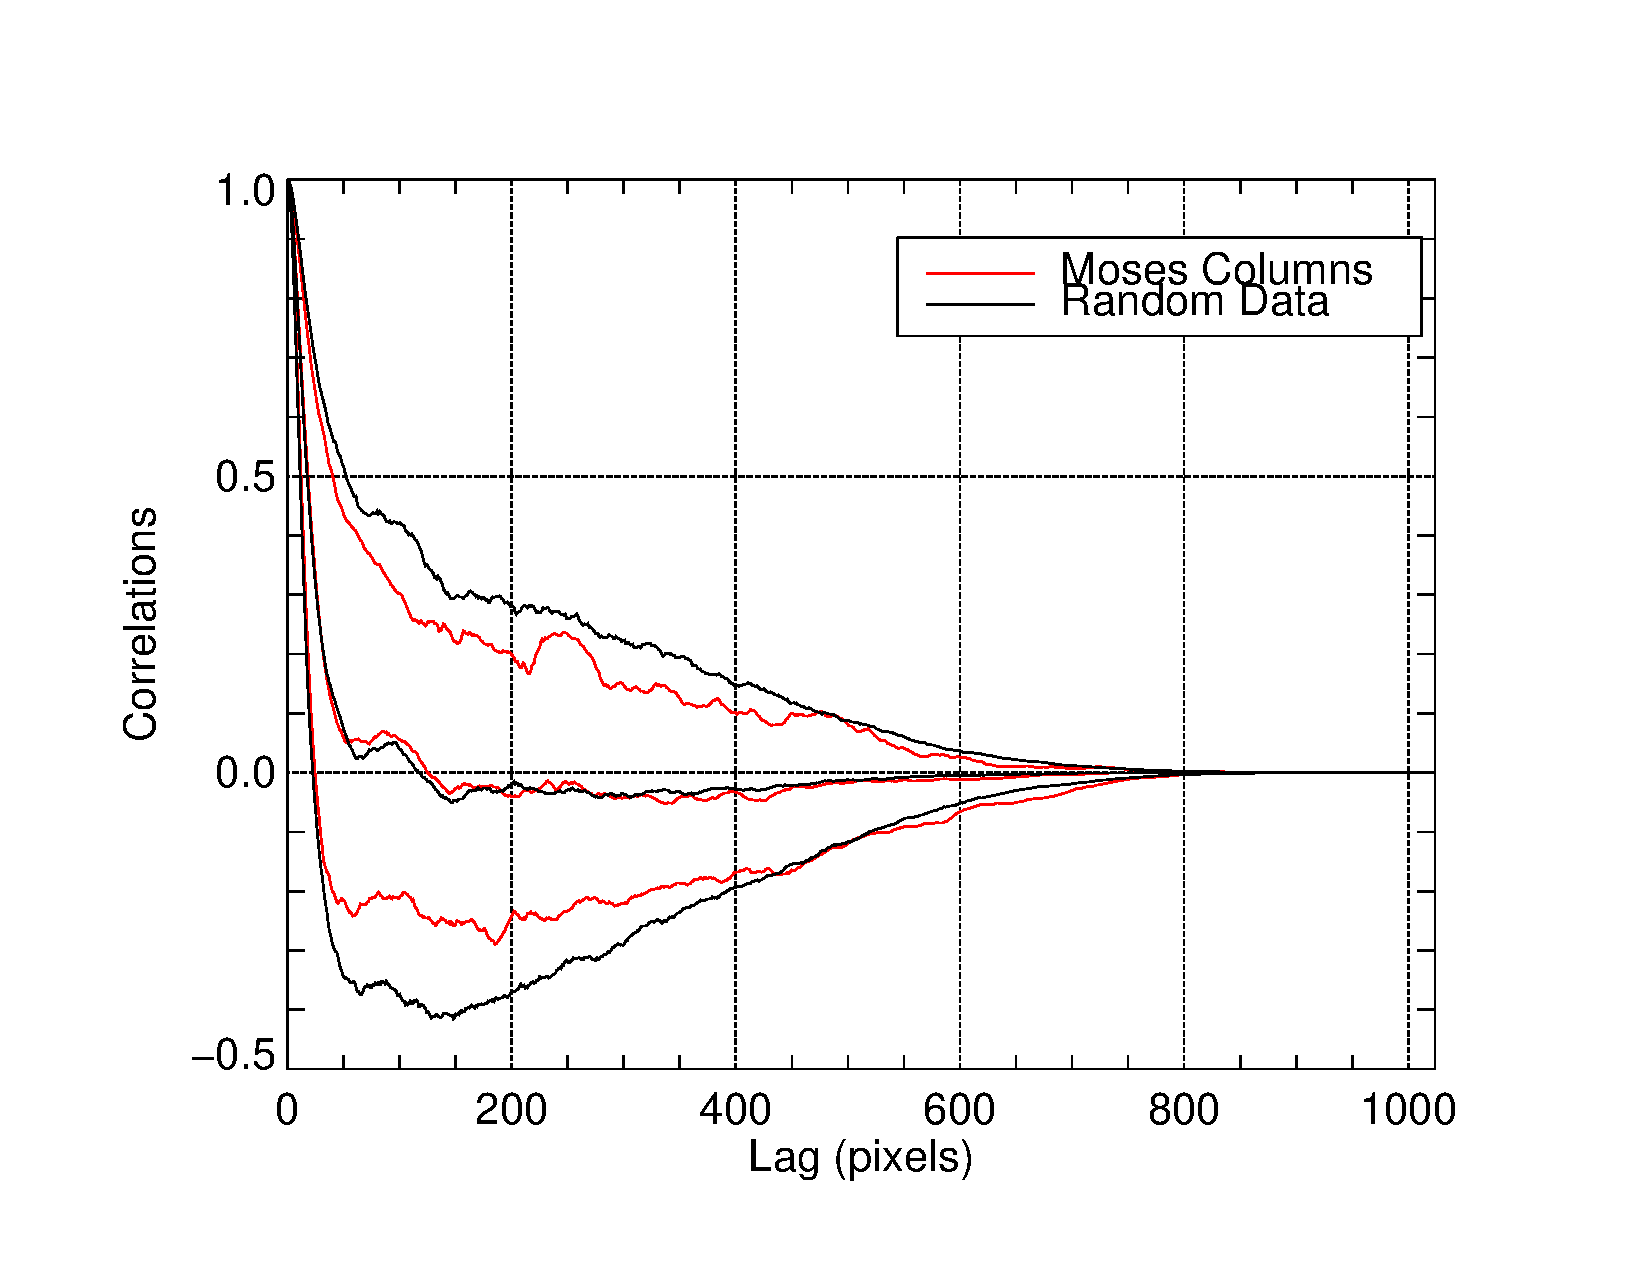
\includegraphics[scale=.5]{images/sigtestauto.pdf}
\caption{A comparison of the auto correlation distribution for \textit{MOSES} columns and random 1024 long section of our random 2048 generated arrays.  The top, middle, and bottom curves define the 93.75th, 50th, and 6.25th percentiles of the distributions.  It has been verified that these curves align for other percentiles as well}
\end{figure*}	

The cross correlation of two subtracted images is non zero for certain lags. Non zero correlation is not necessarily indicative of extra spectral content.   We define confidence intervals for peaks in correlation by producing distributions of correlation at each lag for randomly generated functions.  These random data need to be similar to the actual \textit{MOSES} rows. In order to be a sufficient data set for testing the null hypothesis, that the peaks in correlation aren't significant, these manufactured rows should contain no information about wavelength dispersion.  \textit{MOSES} columns satisfy all of the criteria but are not long enough to investigate correlation at large lag. Therefore part of out random data generation needs to double the array length.

We began our random data generation by widowing the subtracted images in the dispersion dimension.

\begin{equation}
I(x,y) = Hanning(y)*I(x,y)
\end{equation}

Windowing was needed to minimize edge effects.  A FFT , denoted by $\mathcal{F}$, in the vertical dimension transforms the image into an array whose rows are in position space and columns are in Fourier space.

\begin{equation}
\mathcal{F}\lbrace I(x,y) \rbrace = I(x,k_y)
\end{equation}

We Fourier transformed the zero, plus, and minus order images in this fashion.  From these transformed images we can now pick Fourier components at random for our random array. We generate an array of random indices, i, that is 1025 elements long.  Each element of the array is a random number between 0 and 2047. These indices will be the columns from which we pick a value of $k_y$.  This is done for each row j. Row 0 and 512 are the DC and Nyquist frequency terms in the Fourier transform and therefore only need to picked once for the new array. I and j are then used to select Fourier components form each order image to form three new randomly generated arrays.

\begin{equation}
i = floor(randomu(seed,1025)*2047)
\end{equation}
\begin{equation}
j = [0,1,1,2,2,..., 511,511,512]
\end{equation}
\begin{equation}
Random Zero_n = Zero(i_n,j_n)  
\end{equation}
\begin{equation*}
Random Plus_n = Plus(i_n,j_n)   
\end{equation*}
\begin{equation*}
Random Minus_n = Minus(i_n,j_n)   
\end{equation*}
\begin{equation*}
n = 0,1,...,1024
\end{equation*}

Here Zero, Plus, and Minus are used to denote the central, plus, and minus order images.  Random Zero, Random Plus , and Random Minus are arrays with 1025 elements. Since an image is purely real the remaining 1023 elements of the Fourier transform are complex conjugates of those already assigned. The full random array is formed by appending the complex conjugate of the middle 1023 elements to the end of the array in reverse order.

\begin{equation}
Random Plus = [Random Plus,\lbrace reverse(Random Plus(1:1023)\rbrace^*] 
\end{equation}

Using j as described in Equation 5 we double the spectral resolution of each array.  Since the typical power spectrum of a \textit{MOSES} column is relatively smooth we can fill in missing spectral information from a adjacent frequency bin with no issues.  

Figure 6 and 7 show the comparison of \textit{MOSES} data with the random data in both frequency and position space.  Not only do the random data match \MOSES data on average but is also distributed in the same way.  As is noticeable in Figure 7 the data has been windowed with a Hanning window.  This allows us to compare a random 1024 long section of a randomly generated 2048 array. If our method for doubling the array side worked any section of the random array should match the statistics of \MOSES columns. After many iterations of significance testing we are confident that this data is representative of typical solar features observed by \textit{MOSES}.

The confidence intervals in the Figure 5 were generated by sorting the correlation values at a given lag of random subtracted functions.  Our random subtracted images come from subtracting Random Zero from Random Plus and Minus. In the case of the null hypothesis all three orders should be very similar.  The only differences should be from differing point spread function and noise levels.  All arrays are normalized by their median prior to subtraction.

\begin{equation}
PZ =  RandomPlus - RandomZero
\end{equation}
\begin{equation*}
MZ = RandomMinus - RandomZero
\end{equation*}
\begin{equation}
CrossCorrelation (z) = \mathcal{F}^{-1} \lbrace \mathcal{F}(PZ) \mathcal{F}(MZ)^* \rbrace
\end{equation}

Equation 9 shows an alternative way of calculating the Cross Correlation using Fourier Transforms. After a large number of correlation have been computed, 5000 in the case of Figure 5, confidence intervals are defined by removing a percentage, p, of from either end of the distribution for each lag. Here n is the number of degrees of freedom in the system or number of independent events being compared to the random data set.  By picking a confidence level and a representative n we determine what percentage of data, p, to throw out.


\begin{equation}
Confidence = 1-(2p)^n.
\end{equation}

A good indication of the value of n is the correlation length (the lag at which autocorrelation falls to zero and begins random oscillation).  Figure 7 shows that the correlation length is any where from 50 to 150 pixels.  Dividing the number of pixels in a column, 1024, by the correlation length give n from about 7-20.  The significance curves in Figure 5 were plotted using a conservative n=5.

\subsection{Forward Modelling}

Many things contribute to the \MOSES \ cross correlation function beside spectral content.  These complexities make simple forward models fall short in matching our correlation function.  On launch day in 2006 EIT captured full disk images of the sun. These images were captured using the 171 \AA \ , 195 \AA \ , 284 \AA \ , 304 \AA \ filters.  Images from EIT contain all of the complicated spatial information about the Sun on that day. Combinations of these four images can ben used to form fake \MOSES \ data.  We identify the EIT image that best represents each spectral line in the \textit{MOSES} passband by comparing peak line formation temperatures. The image selected for each line is then shifted an amount determined by the instrument dispersion.  Combining these shifted images we create simulated outboard order images.  These can then be subtracted and correlated the same as \textit{MOSES} images.  We can control the resulting cross correlation by changing the line intensity of each image before combination until we get a best fit.  The best fit line intensities will be closest to the spectral content of a \MOSES \ image.


\section{Conclusions}
It is apparent from Figure 5 that peaks in the correlation function of \textit{MOSES} subtracted images are indeed significant.  We have also developed a method for generating random data that is representative of \MOSES \ images. We only applied this method to this specific problem but it could easily be applied to any problem using cross correlations.  

Attempts in fitting the \MOSES \ cross correlation functions have been reasonably successful but still need to be thoroughly explored.  Our forward model does a decent job of fitting behaviour at large lag.  Unfortunately the modelled correlation always peaks at zero lag, unlike the \MOSES \ correlation function.  These peaks straddling zero lag are roughly 10 pixels apart. Because of the narrow peak separation these features are being attributed to smaller, less than 10 pixel, shifts in between orders.  These small shifts could come from imperfections in image alignment, small Doppler shifts, or even differing point spread functions between images.  Figure 8 shows the cross correlation of two subtracted images with small dispersion compared to their size.  For this case the distance between peaks is defined more by object size then dispersion shift.  Hopefully with the addition of \MOSES \ point spread function to our forward model with account for this behaviour and allow for better fitting.

Regardless of difficulties in fitting small lag features a well tuned forward model will give us an idea of how much extra spectral content exist in \MOSES \ images.  This information will improve our ability to invert current and future \MOSES \ data sets.  These measurements should also stand as a warning for anyone trying to determine solar parameters from He II passband images.  Despite the fact that He II images are dominated by transition features they contain a fair about of coronal influence.



\begin{figure*}[t]
\figurenum{8}
\centering
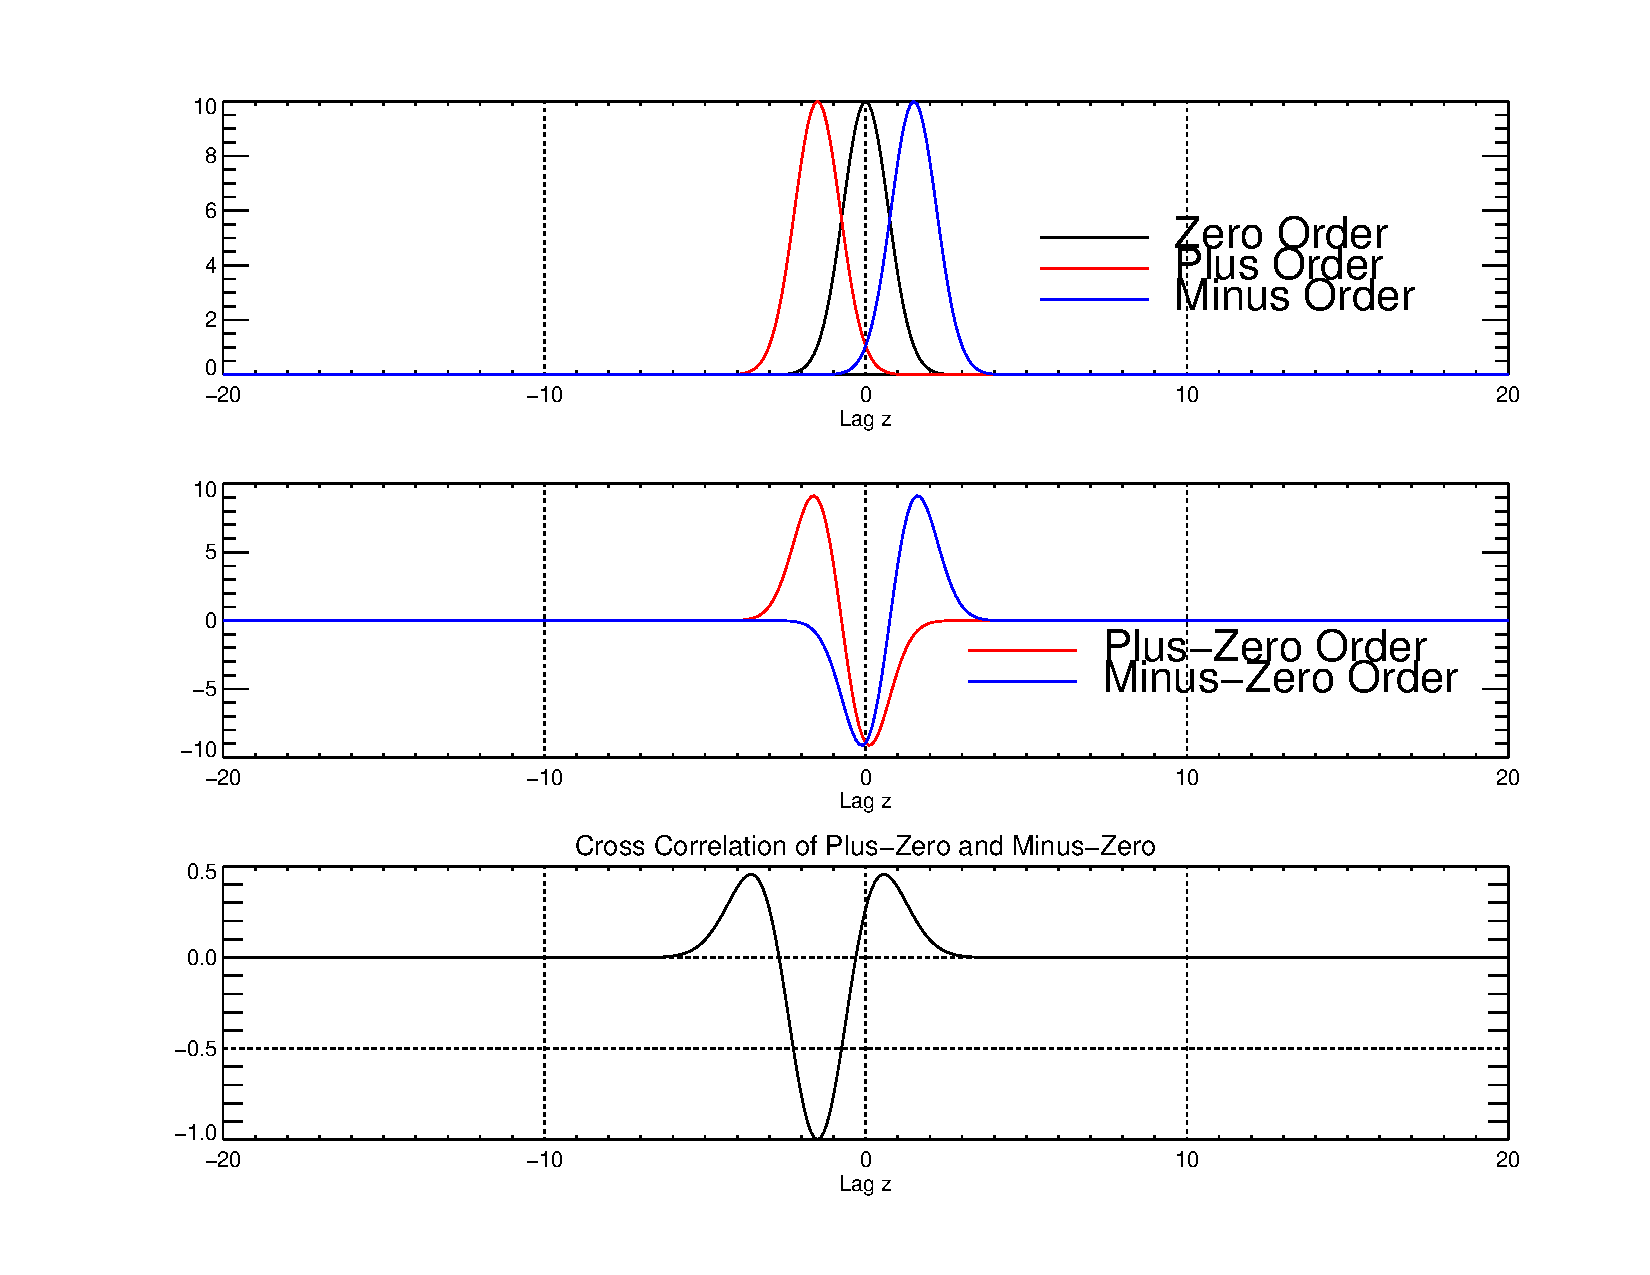
\includegraphics[scale=.5]{images/test2.pdf}
\caption{An example of the correlation function generated by an object that has a size in pixels that is close to its dispersion in pixels.  The cross correlation function of the two subtracted functions no longer peaks at zero}
\end{figure*}	




\begin{thebibliography}{}

\bibitem[Kankelborg et al.(2001)]{Kan01} Charles C. Kankelborg ; Roger J. Thomas; Simultaneous imaging and spectroscopy of the solar atmosphere: advantages and challenges of a 3-order slitless spectrograph. Proc. SPIE 4498, UV/EUV and Visible Space Instrumentation for Astronomy and Solar Physics, 16 (December 10, 2001); doi:10.1117/12.450074.

\bibitem[Brosius et al.(1998)]{Spec98} Jeffrey W. Brosius et al 1998 ApJS 119 255

\bibitem[Owens et al.(2005)]{Owens2005}  Scott M. Owens, Jeffery S. Gum, Charles Tarrio, et al., "Narrow-band EUV multilayer coating for the MOSES sounding rocket", Proceedings of SPIE Vol. 5900, 590003 (2005)   SPIE 




\end{thebibliography}{}	
	
\end{document}
	
